\chapter{A térkép}
A pálya aktuális térképe a \ref{fig:stalingrad}. ábrán látható.

\begin{figure}
    \centering
    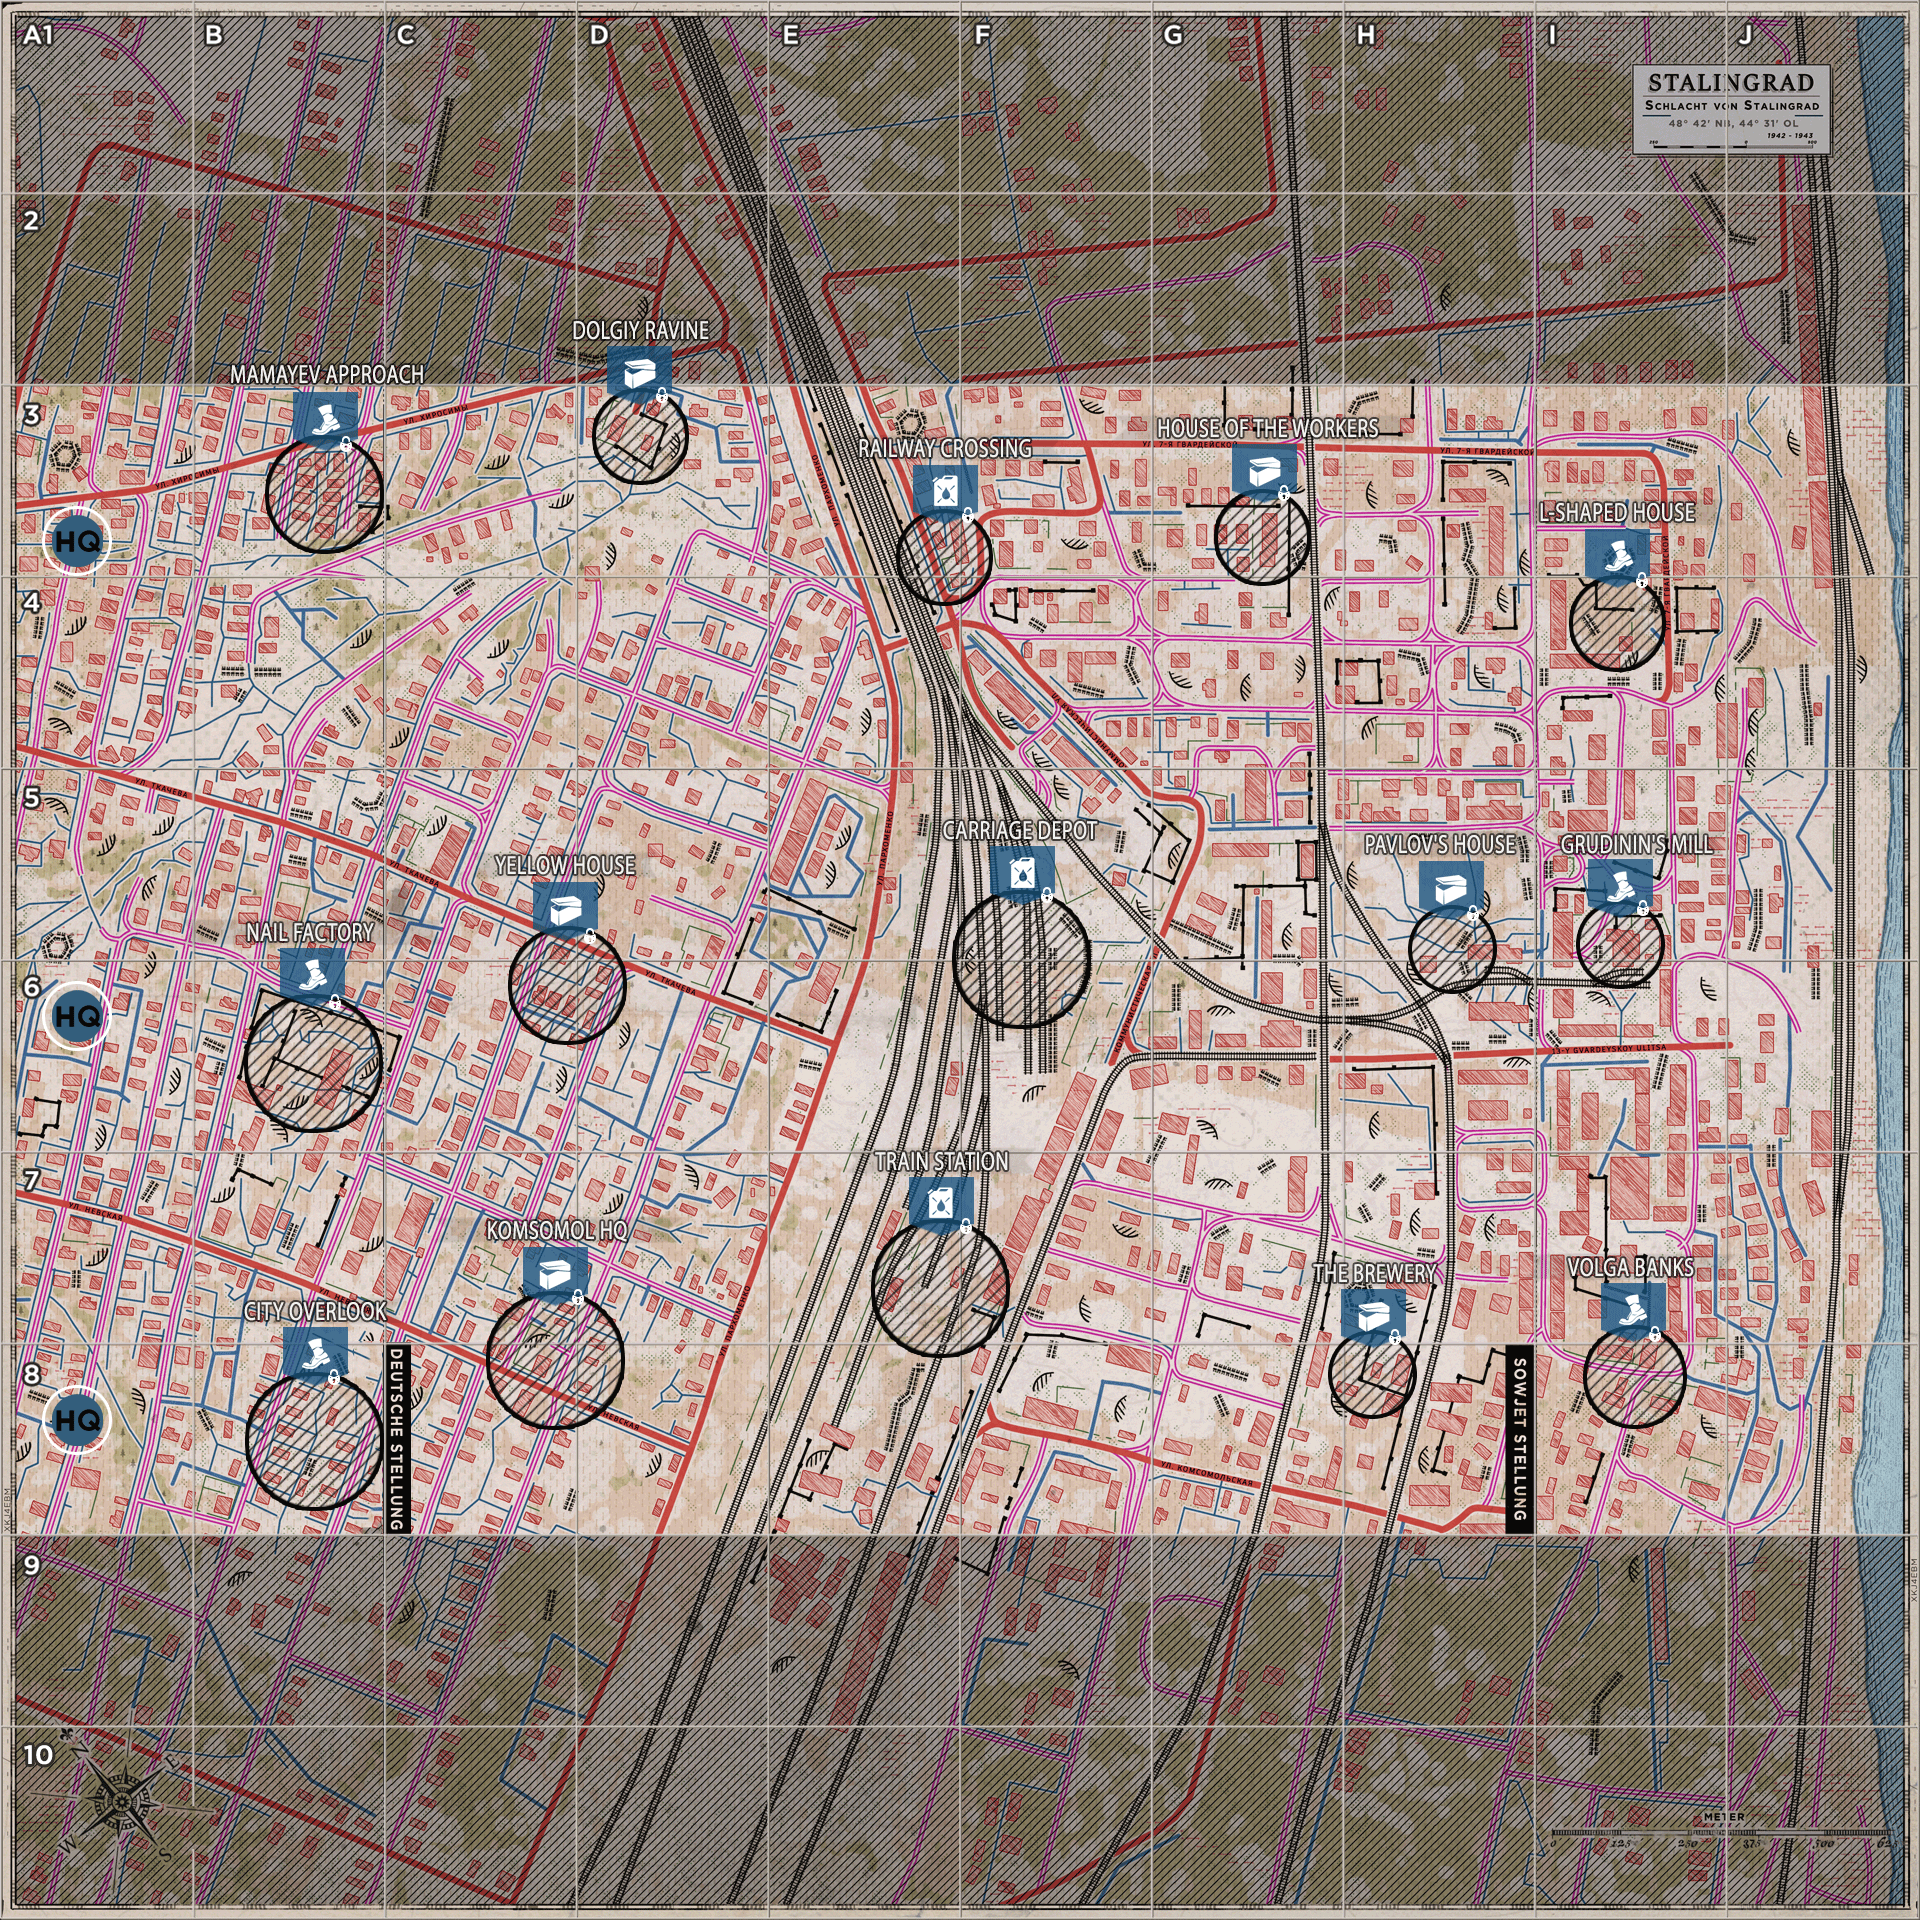
\includegraphics[width=150mm, keepaspectratio]{figures/StalingradMap.png}
    \caption{Sztálingrád térképe}
    \label{fig:stalingrad}
\end{figure}

%-------------------------------------
\section{Német bázis sáv}
%-------------------------------------
\subsection{Mamayev Approach}

\subsection{Nail Factory}

\subsection{City Overlook}

%-------------------------------------
\section{Német védekező sáv}
%-------------------------------------
\subsection{Dolgiy Ravine}

\subsection{Yellow house}

\subsection{Komsomol HQ}

%-------------------------------------
\section{Semleges sáv}
%-------------------------------------
\subsection{Railway Crossing}

\subsection{Carriage Depot}

\subsection{Train Station}

%-------------------------------------
\section{Orosz védekező sáv}
%-------------------------------------
\subsection{House of the Workers}

\subsection{Pavlov's House}

\subsection{The Brewery}

%-------------------------------------
\section{Orosz bázis sáv}
%-------------------------------------
\subsection{L-Shaped House}

\subsection{Grudinin's Mill}

\subsection{Volga Banks}